\chapter{Vaja: politika}
\label{hw:grucenje}

Čas je, da preizkusimo novo znanje. V gradniku \widget{File} z namizja naložite podatke \textit{slovenski-parlament.tab}.

\hspace{1cm}

1. Z Box Plotom ugotovite, kakšna je povprečna starost poslancev.

\begin{marginfigure}
    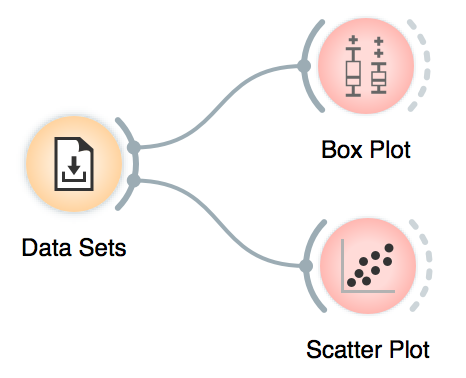
\includegraphics[scale=0.6]{workflow1.png}
    \caption{$\;$}
\end{marginfigure}

2. S Scatter Plotom odkrijte, kdo največ govori na sejah parlamenta (ima največ govorov na sejo in besed na sejo). Zakaj je tako?

3. V Scatter Plotu pripravite vizualizacijo prisotnosti poslancev na sejah in njihovih pobud. Kaj lahko ugotovite iz teh dveh spremenljivk?

\hspace{1cm}

Čas je, da ugotovimo, kateri poslanci so si med sabo najbolj podobni. Računali bomo zgolj razdaljo med glasovanjem poslancev na sejah parlamenta. Najprej moramo izmeriti razdalje med njimi in uporabiti hierarhično razvrščanje, da odkrijemo skupine. Ročno izberite število skupin tako, da povlečete razmejitveno črto levo ali desno v vizualizaciji.

\begin{figure}[h]
    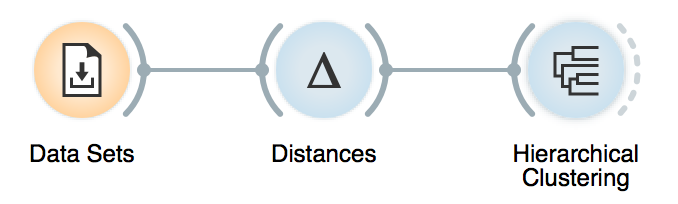
\includegraphics[scale=0.6]{workflow2.png}
    \caption{$\;$}
\end{figure}

4. Kakšno bi bilo primerno število skupin? Kako bi interpretirali te skupine? Zapišite predlagano število skupin in ključno lastnost posamezne skupine (po čem so si poslanci podobni).

\hspace{1cm}

\begin{wrapfigure}{o}{1.1\textwidth}
    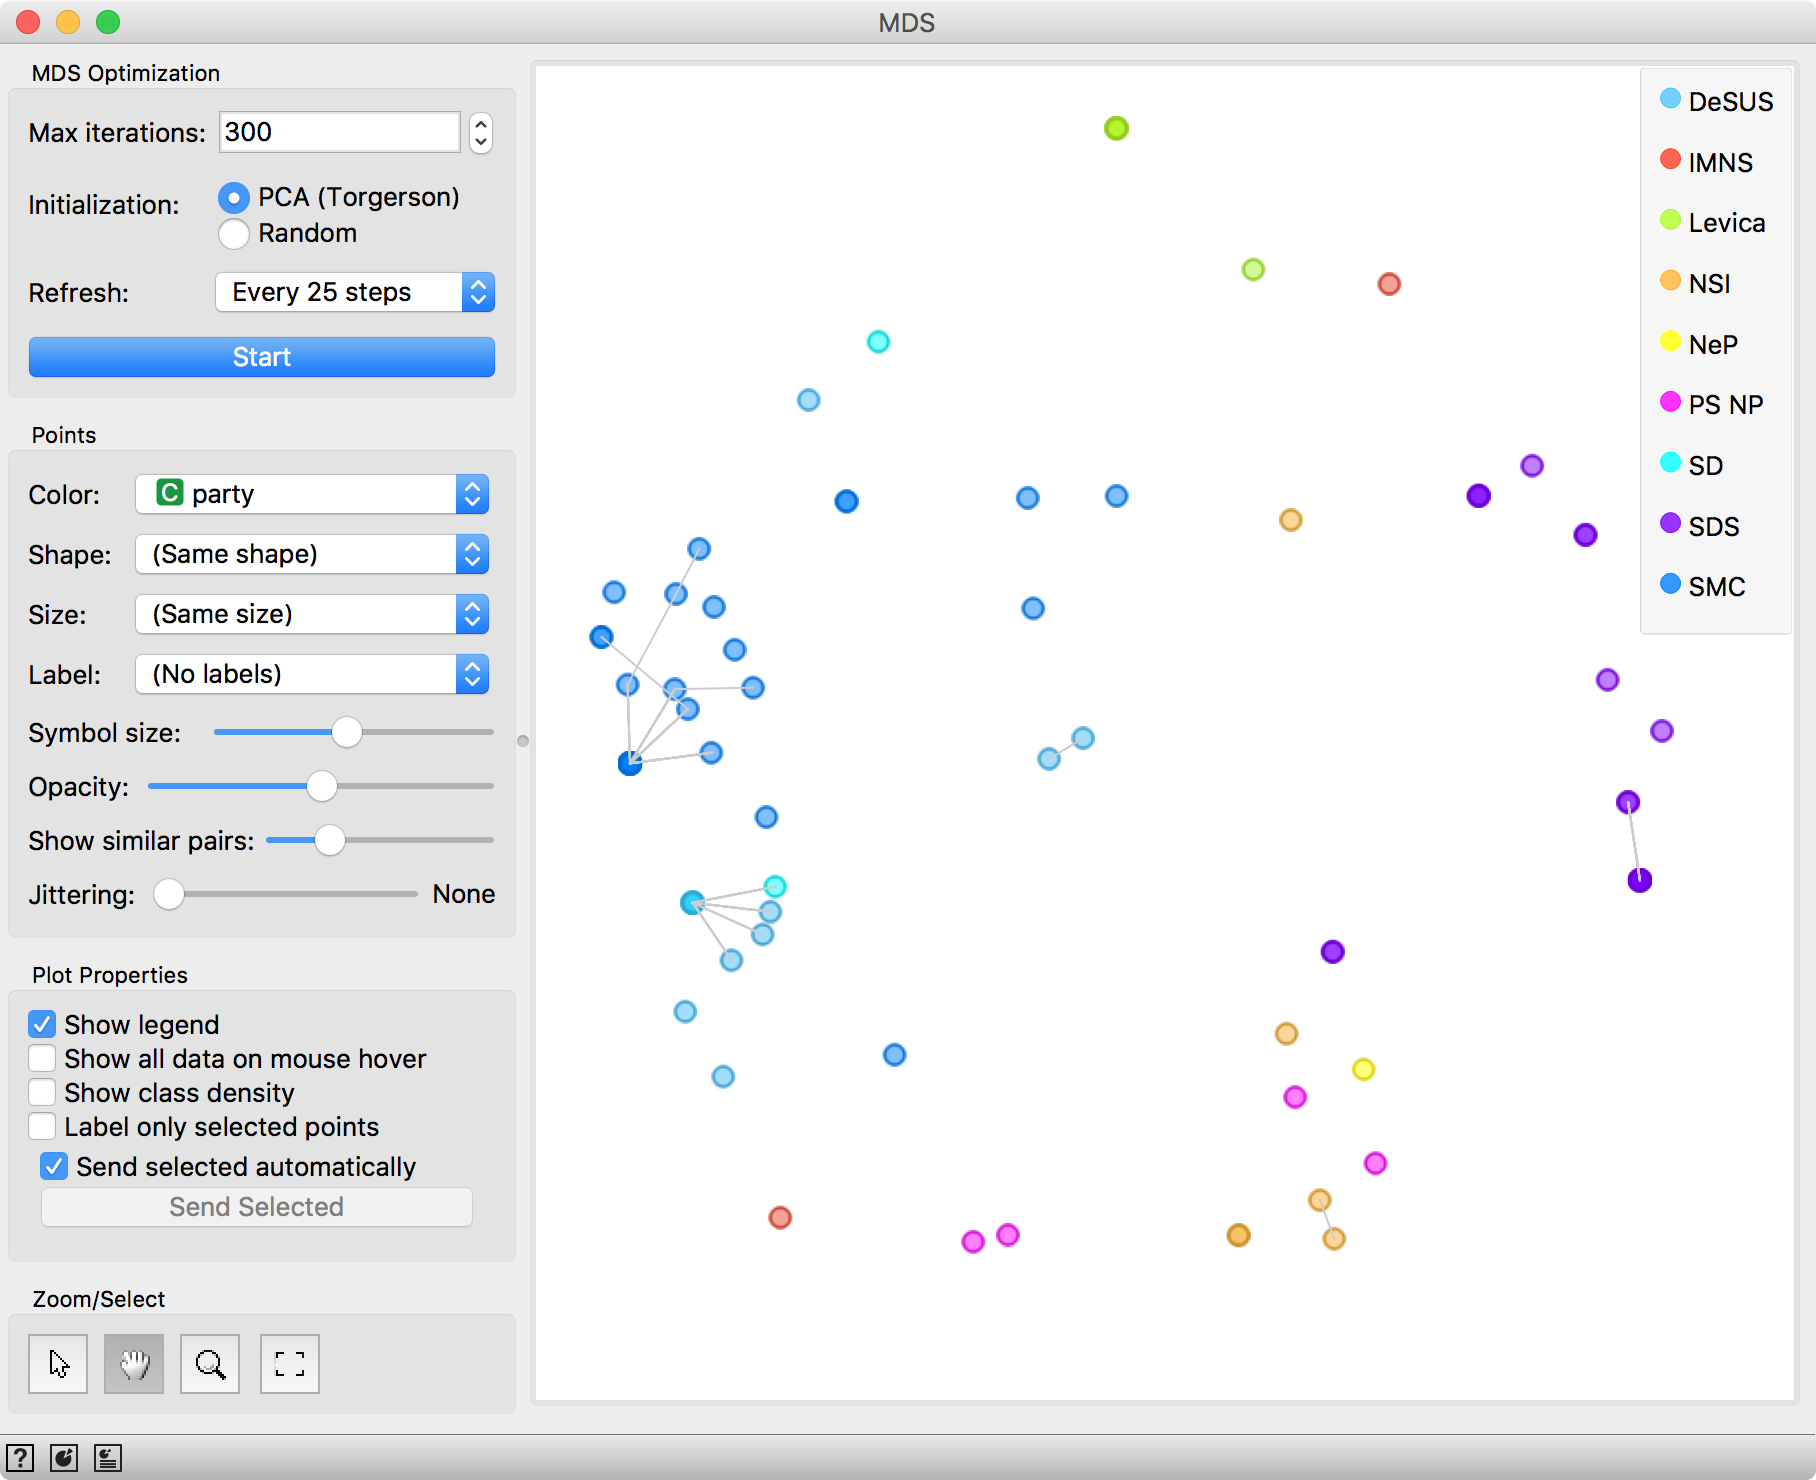
\includegraphics[scale=0.35]{mds.png}
    \caption{$\;$}
\end{wrapfigure}

Iz dendrograma težko ugotovimo, kako blizu si je naključen par poslancev. Z vizualizacijo MDS bomo prikazali poslance tako, da bodo podobni poslanci blizu skupaj. Dobili bomo nekakšen zemljevid poslancev.

\hspace{1cm}

5. Kateri poslanec glasuje izrazito drugače kot njegova stranka?
